\documentclass[12pt]{beamer}

\usepackage[utf8]{inputenc} % un package
\usepackage[francais]{babel}  % un troisième package
\usepackage{graphicx}
\usepackage{fancybox}
\usepackage{listings}
\usepackage{color}
 
\definecolor{dkgreen}{rgb}{0,0.6,0}
\definecolor{mauve}{rgb}{0.58,0,0.82}
 
\lstset{ %
	language=sh,                % the language of the code
  basicstyle=\tiny,           % the size of the fonts that are used for the code
  numbers=left,                   % where to put the line-numbers
  numberstyle=\footnotesize,          % the size of the fonts that are used for the line-numbers
  stepnumber=1,                   % the step between two line-numbers. If it's 1, each line 
                                  % will be numbered
  numbersep=5pt,                  % how far the line-numbers are from the code
  backgroundcolor=\color{white},      % choose the background color. You must add \usepackage{color}
  showspaces=false,               % show spaces adding particular underscores
  showstringspaces=false,         % underline spaces within strings
  showtabs=false,                 % show tabs within strings adding particular underscores
  frame=single,                   % adds a frame around the code
  tabsize=2,                      % sets default tabsize to 2 spaces
  captionpos=b,                   % sets the caption-position to bottom
  breaklines=true,                % sets automatic line breaking
  breakatwhitespace=false,        % sets if automatic breaks should only happen at whitespace
  title=\lstname,                   % show the filename of files included with \lstinputlisting;
                                  % also try caption instead of title
  numberstyle=\tiny\color{red},        % line number style
  keywordstyle=\color{blue},          % keyword style
  commentstyle=\color{dkgreen},       % comment style
  stringstyle=\color{mauve},         % string literal style
  escapeinside={\%*}{*)},            % if you want to add a comment within your code
  morekeywords={mkdir,hg}               % if you want to add more keywords to the set
}
\setbeamertemplate{blocks}[rounded][shadow=true]

\usetheme{Berlin}
\setbeamercovered{highly dynamic}
\title[Galaxy]{Analyse technique de logiciel\\ Galaxy}
\author[F. C. | B. D. | S. B. | G. B. | T. L.]{Florian CARRE\\Benjamin DARTIGUES\\Sebastien BEAUQUIS\\Guillaume BERNARD\\Tom LESLUYES}
\date{30 Janvier 2012}
\institute[]{Université de Bordeaux 1}


\begin{document}
\maketitle

\section*{Sommaire}
\begin{frame}
\frametitle{Sommaire}
\tableofcontents[pausesections]
\end{frame}

%%%%%%%%%%%%%%%%%%%%%%%%%%%%%%%%%%%%%%
%%%%%%%%%%%%%%%%%%%%%%%%%%%%%%%%%%%%%%%
\section{Etat de l'art}
\begin{frame}{les logiciels de worflow}
\begin{block}{Présentation générales}
On distingue deux types de logiciels de workflow : 
\begin{itemize}
 \item les logiciels de workflow 1
\item les logiciels de workflow 2
\end{itemize}
\end{block}
\end{frame}


\subsection{Les logiciels de workflow }
\begin{frame}{les logiciels de worflow 1}
\begin{block}{Ergatis, BIOMOBY}
\begin{itemize}
 \item Ergatis
\item BIOMOBY
\end{itemize}
\end{block}
\end{frame}



\section{NGS : Next Generation Sequencing}
\begin{frame}{NGS}
\begin{block}{Présentation des techniques de NGS}
\begin{itemize}
 \item la technique 454 : le pyrosequençage
\item la méthode de sequençage Illumina.
\end{itemize}
\end{block}
\end{frame}

\subsection{Pyroséquençage}
\begin{frame}{Le pyrosequençage}
\begin{center}
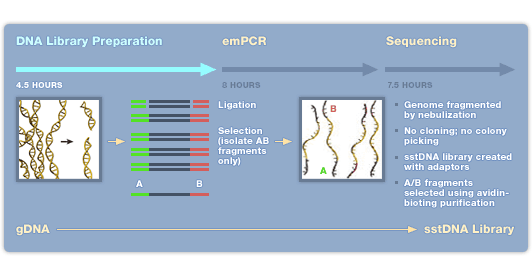
\includegraphics[scale=0.6]{./img/seq1.png}
\end{center}
\end{frame}


\begin{frame}{Le pyrosequençage}
\begin{center}
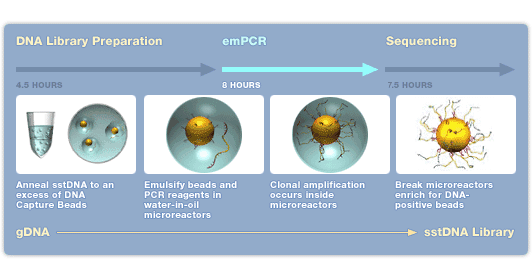
\includegraphics[scale=0.6]{./img/microbille.png}
\end{center}
\end{frame}


\begin{frame}{Le pyrosequençage}
\begin{center}
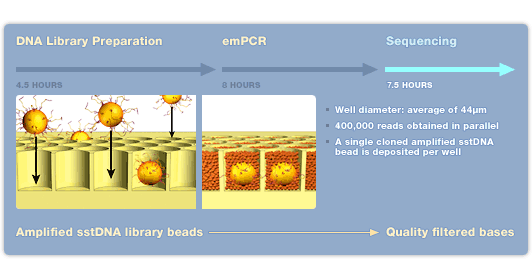
\includegraphics[scale=0.6]{./img/incbil.png}
\end{center}
\end{frame}


\begin{frame}{Le pyrosequençage}
\begin{center}
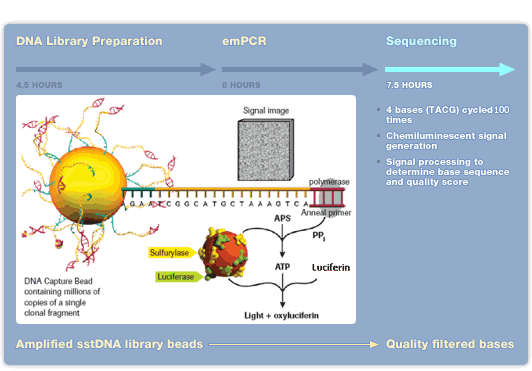
\includegraphics[scale=0.48]{./img/sequ454.png}
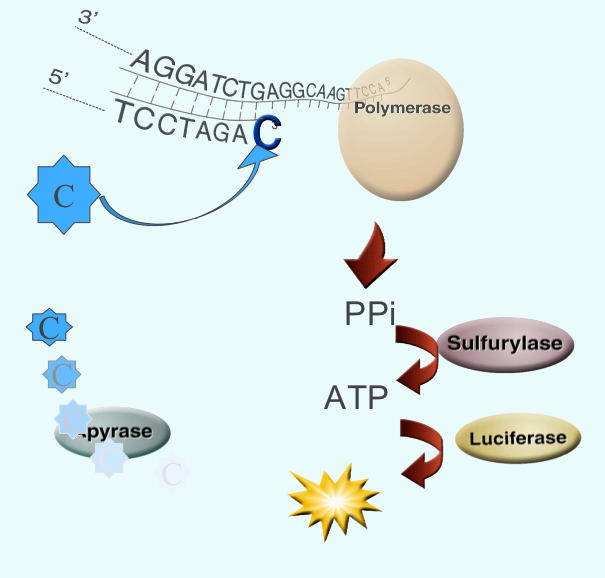
\includegraphics[scale=0.3]{./img/proces.png}
\end{center}
\end{frame}


\begin{frame}{Le pyrosequençage}
\begin{center}
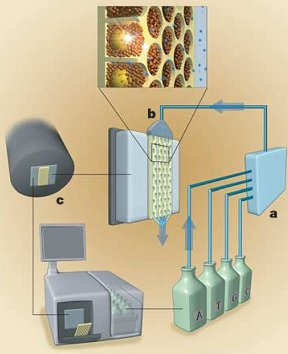
\includegraphics[scale=0.5]{./img/mach.png}

\includegraphics[scale=0.59]{./img/454.png}
\end{center}
\end{frame}

\subsection{Illumina}
\begin{frame}{Illumina}
\begin{center}
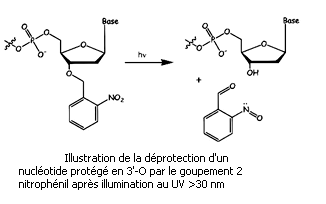
\includegraphics[scale=0.65]{./img/react.png}
\end{center}
\begin{block}{De Sanger à Illumina}
CRT : Cycle Reversible Termination
\end{block}
\end{frame}

\begin{frame}{Illumina}
\begin{minipage}{0.49\textwidth}
\begin{flushright}
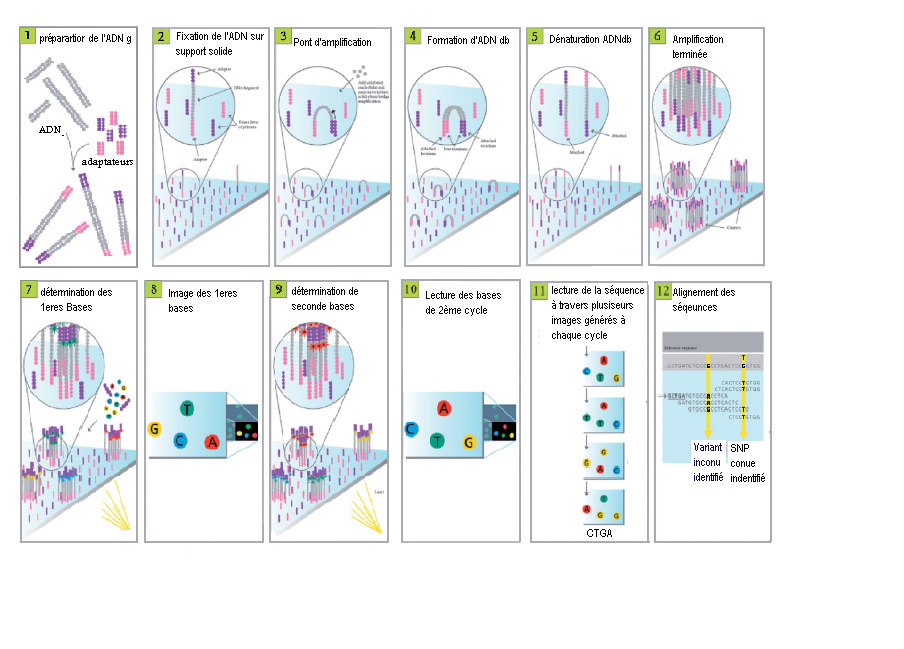
\includegraphics[scale=0.33]{./img/sequfr1.png}
\end{flushright}
\end{minipage}
\end{frame}

\section{Utilisation}

\begin{frame}{Trois types d'utilisation différentes}
\begin{block}{}
\begin{itemize}
\item Utilisation en ligne.
\item Utilisation en local.
\item Utilisation sur un "cloud".
\end{itemize}
\end{block}
\end{frame}

\subsection{Utilisation en ligne}
\begin{frame}{Avantages et inconvénient}
\begin{columns}
\begin{column}{0.5\textwidth}
\begin{block}{Avantages de l'utilisation en ligne}
\begin{itemize}
\item Aucune installation nécessaire.
\item Interface ergonomique.
\item Nombreux "tutoriels" et aides.
\end{itemize}
\end{block}
\end{column}
\begin{column}{0.5\textwidth}
\begin{block}{Inconvénient de l'utilisation en ligne}
\begin{itemize}
\item Connexion internet requise.
\end{itemize}
\end{block}
\end{column}
\end{columns}
\end{frame}

\begin{frame}{Interface graphique}
\scriptsize
\center{
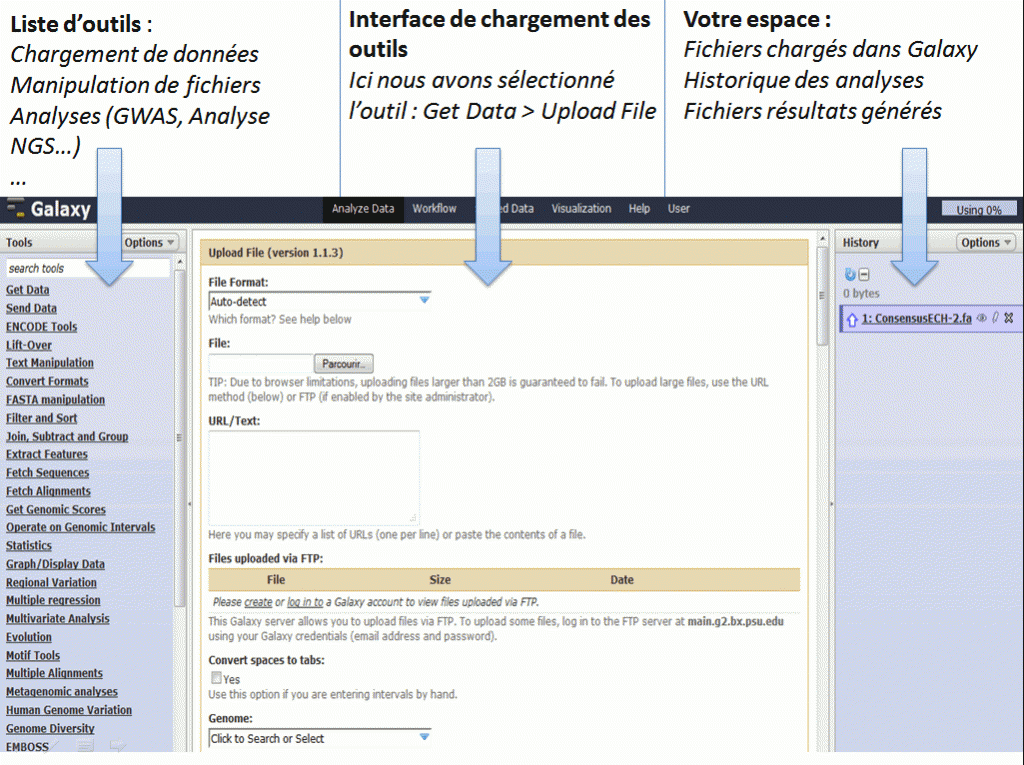
\includegraphics[width=8cm]{img/interface.png}\\
}
\end{frame}

\begin{frame}{Page d'aide d'un des outils de Galaxy}
\scriptsize
\center{
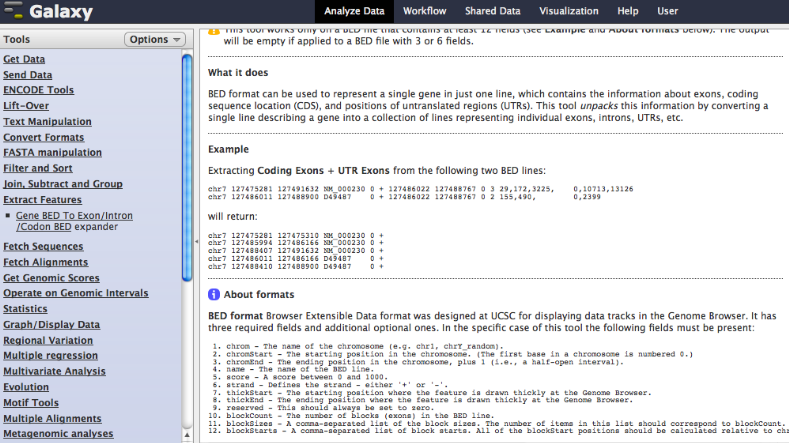
\includegraphics[width=10cm]{img/exinfo.png}\\
}
\end{frame}

\subsection{Utilisation en local}
\begin{frame}{Avantages et Inconvénient}
\begin{columns}
\begin{column}{0.5\textwidth}
\begin{block}{Avantages de l'utilisation en local}
\begin{itemize}
\item Ne nécessite pas de connexion internet.
\item Possibilité de modifier les paramêtres des plug-ins.
\item Possibilité d'ajouter des plug-ins.
\item Vitesse d'analyse.
\item Conservation des données sensibles.
\end{itemize}
\end{block}
\end{column}
\begin{column}{0.5\textwidth}
\begin{block}{Inconvénient de l'utilisation en local}
\begin{itemize}
\item Installation nécessaire.
\end{itemize}
\end{block}
\end{column}
\end{columns}
\end{frame}

\begin{frame}{Téléchargement du code source}
\begin{block}{}
\begin{itemize}
\item Récupération de la dernière version de Galaxy depuis Bitbucket.
\item Téléchargement du répertoire Galaxy à partir de Mercurial.
\end{itemize}
\end{block}
\end{frame}

\begin{frame}{Récupération à partir de  Mercurial}
\begin{block}{Commandes pour copier le répertoire}
mkdir Galaxy\\
cd Galaxy\\
hg clone https://bitbucket.org/galaxy/galaxy-dist/\\
\end{block}
\begin{block}{Commandes pour effectuer les mises à jour}
hg incoming\\
hg pull -u\\
\end{block}
\end{frame}

\begin{frame}{Exécution du serveur local}
\begin{block}{Commandes pour exécuter le script \textit{run.sh}}
sh run.sh   \# commande de base\\
sudo run.sh   \# commande administrateur\\
\end{block}
\begin{block}{Adresse du serveur de Galaxy}
\scriptsize
\center{

\includegraphics[width=8cm]{img/Adresselocale.png}\\
}
\end{block}
\end{frame}

\begin{frame}{Exécution du serveur local}
\scriptsize
\center{
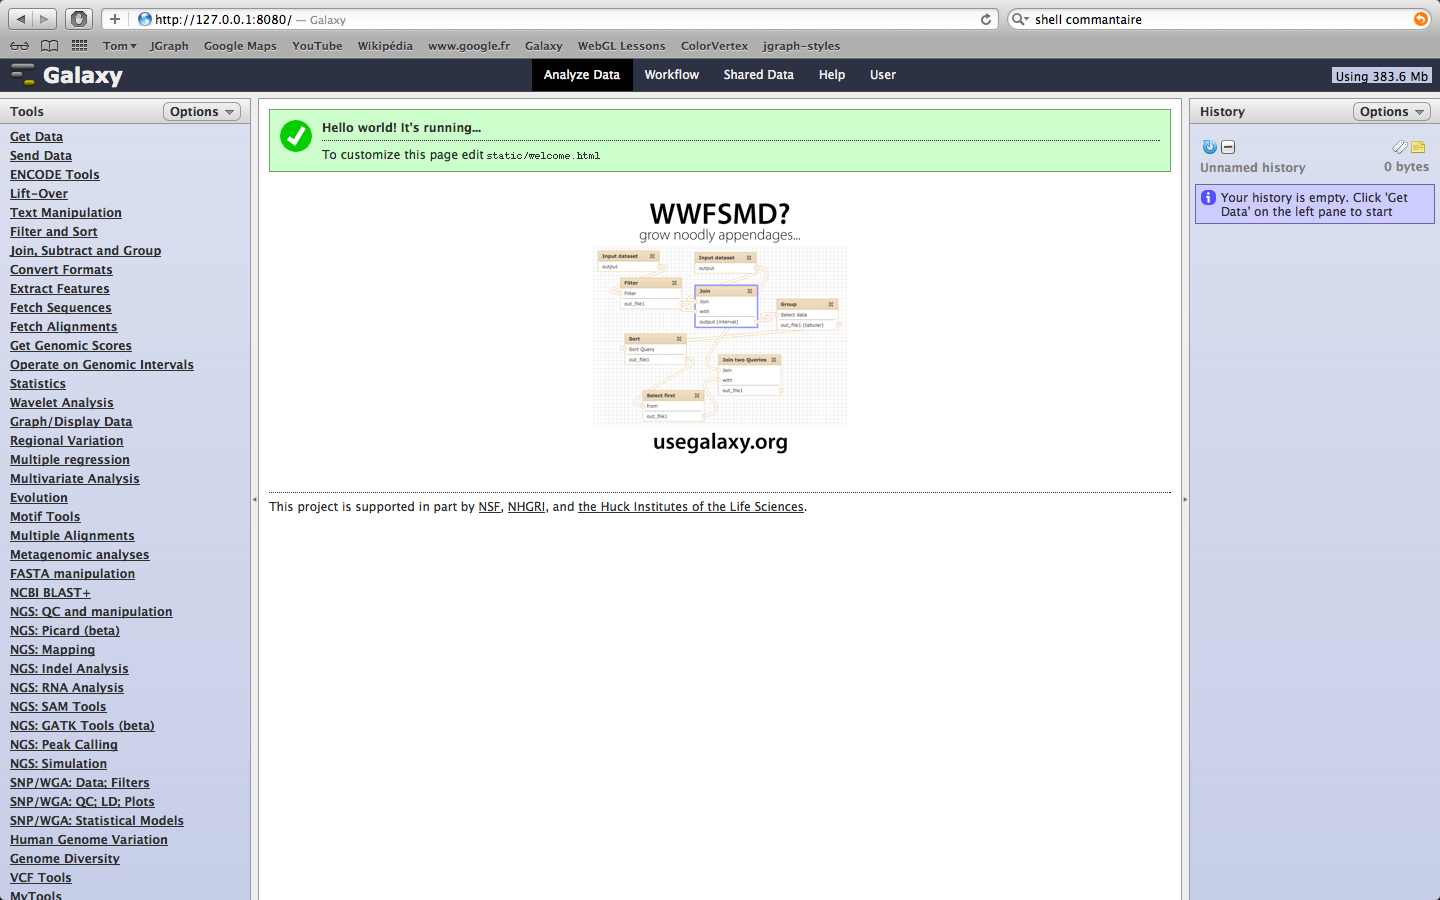
\includegraphics[width=9cm]{img/Galaxylocal.png}\\
}
\end{frame}

\section{Fonctionnalités}
\begin{frame}
\frametitle{Fonctionnalités}
\begin{block}{Très nombreuses}
\begin{itemize}
\pause
\item Présentation générale
\item Ajout de plug-ins
\item Workflow
\end{itemize}
\end{block}
\end{frame}
\subsection{Présentation générale}
\begin{frame}
\frametitle{Présentation générale}
\begin{block}{Pré-traitement}
\begin{itemize}
\item Manipulation de fichiers
	\begin{itemize}
	\item ouverture de fichiers volumineux
	\item ajout/suppression de lignes
	\item concaténation, filtrage, intersection
	\item etc ...
	\end{itemize}
	\pause
\item Opérations sur les données
	\begin{itemize}
	\item addition, soustraction, moyenne, calcul de taille de séquences
	\item conversion, formatage
	\item etc ...
	\end{itemize}
\end{itemize}

\end{block}
\end{frame}
\begin{frame}
\begin{block}{Traitement}

\begin{itemize}
\frametitle{Présentation générale}
\item Analyse de séquences
	\begin{itemize}
	\item calcul de corrélation
	\item recherche d'orthologues
	\item utilisation des outils d'EMBOSS
	\item etc ...
	\end{itemize}
	\pause
\item Visualisation des données
	\begin{itemize}
	\item alignements multiples
	\item distribution de données (histogramme, scatterplot)
	\item arbres phylogéniques
	\item etc ...
	\end{itemize}
\end{itemize}

\end{block}
\end{frame}

\subsection{Ajout de plug-ins}
\begin{frame}
\frametitle{Ajout de plug-ins}
	\begin{itemize}
	\item Instance locale
	\item Langages interprétés
	\item Langages compilés
	\end{itemize}
\only<2>{
  \begin{block}{}
  \begin{figure}
   \begin{center}
    
\includegraphics[scale=0.15]{img/Logopython.png} \textbf{}
    
\includegraphics[scale=0.15]{img/Logoruby.png} \textbf{}
    
\includegraphics[scale=0.15]{img/Logoperl.png} \textbf{}
   \end{center}
  
  \end{figure}
  \begin{figure}
   \begin{center}
    
\includegraphics[scale=0.15]{img/Logoc.png} \textbf{}
    
\includegraphics[scale=0.15]{img/Logocpp.png} \textbf{}
    
\includegraphics[scale=0.15]{img/Logojava.png} \textbf{}
   \end{center}
  
  \end{figure}
\end{block}
}
\end{frame}

\begin{frame}[fragile]
\frametitle{Calcul du GC\% à l'aide d'un script Perl}
\lstset{language=Perl}
\begin{lstlisting}
#!/usr/bin/perl -w
open (IN, "<$ARGV[0]");
open (OUT, ">$ARGV[1]");
while (<IN>) {
    chop;
    if (m/^>/) {
        s/^>//;
        if ($. > 1) {
            print OUT sprintf("%.3f", $gc/$length) . "\n";
        }
        $gc = 0;
        $length = 0;
    } else {
        ++$gc while m/[gc]/ig;
        $length += length $_;
    }
}
print OUT sprintf("%.3f", $gc/$length) . "\n";
close( IN );
close( OUT );
 \end{lstlisting} 
\end{frame}

\begin{frame}[fragile]
\frametitle{\textit{tool\_conf.xml}}
\lstset{language=XML}
\begin{lstlisting}[morekeywords={section,tool},basicstyle=\small,numberstyle=\scriptsize\color{red}]
<section name="MyTools" id="mTools">
    <tool file="myTools/toolExample.xml" />
 </section>
 \end{lstlisting} 
\end{frame}
\begin{frame}[fragile]
\frametitle{\textit{toolExample.xml}}
\lstset{language=XML}
\begin{lstlisting} [morekeywords={description,command,inputs,param,inputs,input,output,outputs,data,tests,test,help,tool}]
<tool id="fa_gc_content_1" name="Compute GC content">
  <description>for each sequence in a file</description>
  <command interpreter="perl">toolExample.pl $input $output</command>
  <inputs>
    <param format="fasta" name="input" type="data" label="Source file"/>
  </inputs>
  <outputs>
    <data format="tabular" name="output" />
  </outputs>
  <tests>
    <test>
      <param name="input" value="fa_gc_content_input.fa"/>
      <output name="out_file1" file="fa_gc_content_output.txt"/>
    </test>
  </tests>
  <help>
This tool computes GC content from a FASTA file.
  </help>
</tool>
 \end{lstlisting}
\end{frame}

\begin{frame}
\begin{center}

\frametitle{Outil implémenté}
\begin{columns}
\begin{column}{5cm}
  \begin{figure}
   \begin{center}
 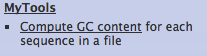
\includegraphics[scale=0.5]{img/Ongletmytools.png}
 	\caption{Ajout du script dans la liste d'outils}
   \end{center}
  \end{figure}
  \end{column}
  \begin{column}{5cm}
  \begin{figure}
   \begin{center}
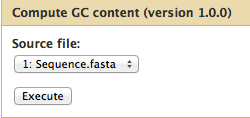
\includegraphics[scale=0.4]{img/Gccontent.png}
   	\caption{Fichier d'entrée}

   	\end{center}
  \end{figure}
  \end{column}
\end{columns}
\begin{figure}
   \begin{center}
 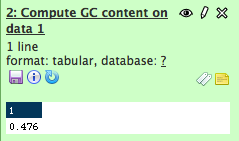
\includegraphics[scale=0.4]{img/Resultatgc.png}
 	\caption{Résultat}
   \end{center}
  \end{figure}
\end{center}
\end{frame}

\subsection{Workflow}
\begin{frame}
\frametitle{Exemple de workflow}
\begin{figure}
   \begin{center}
 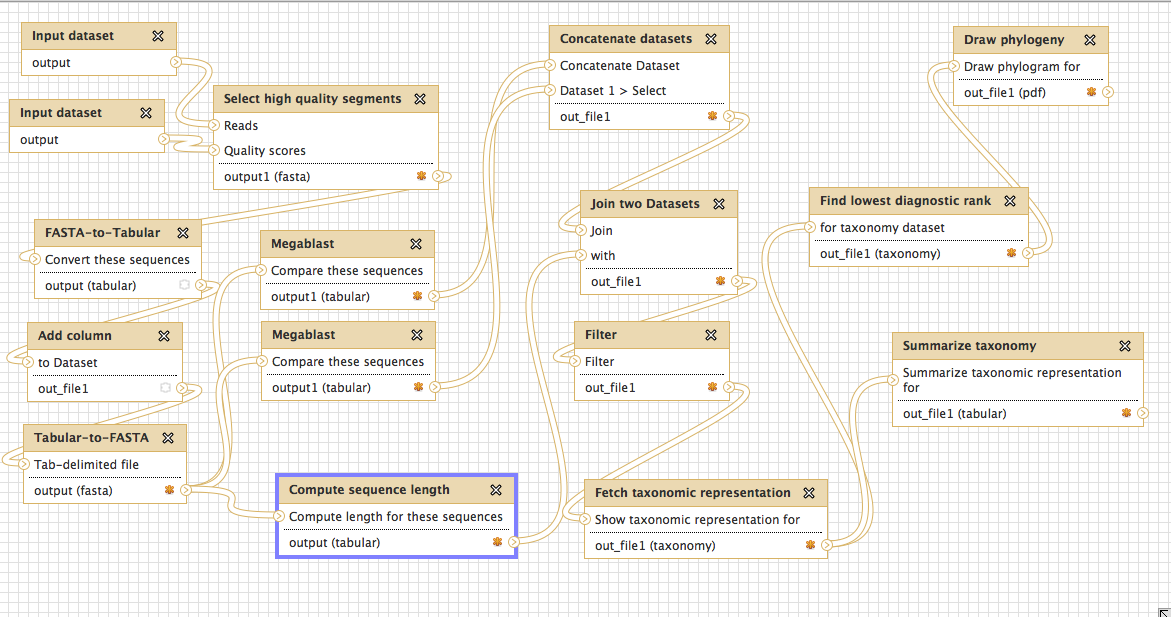
\includegraphics[scale=0.23]{img/workflow1.png}
 	\caption{Workflow de métagénomique}
   \end{center}
  \end{figure}
\end{frame}

\begin{frame}
\frametitle{Lancement de workflow}
\begin{figure}
   \begin{center}
 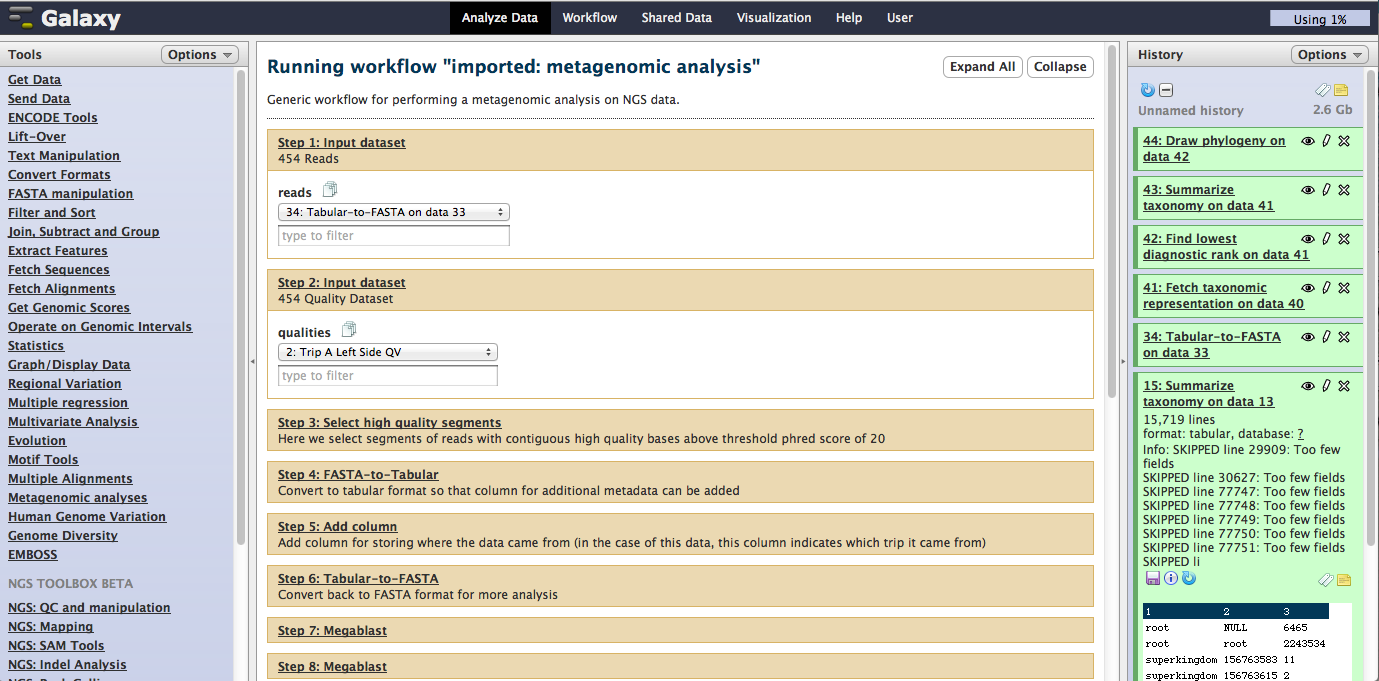
\includegraphics[scale=0.2]{img/preRun.png}
 	\caption{Lancement du workflow}
   \end{center}
  \end{figure}
\end{frame}

\begin{frame}
\frametitle{Résultat du workflow}
\begin{figure}
   \begin{center}
 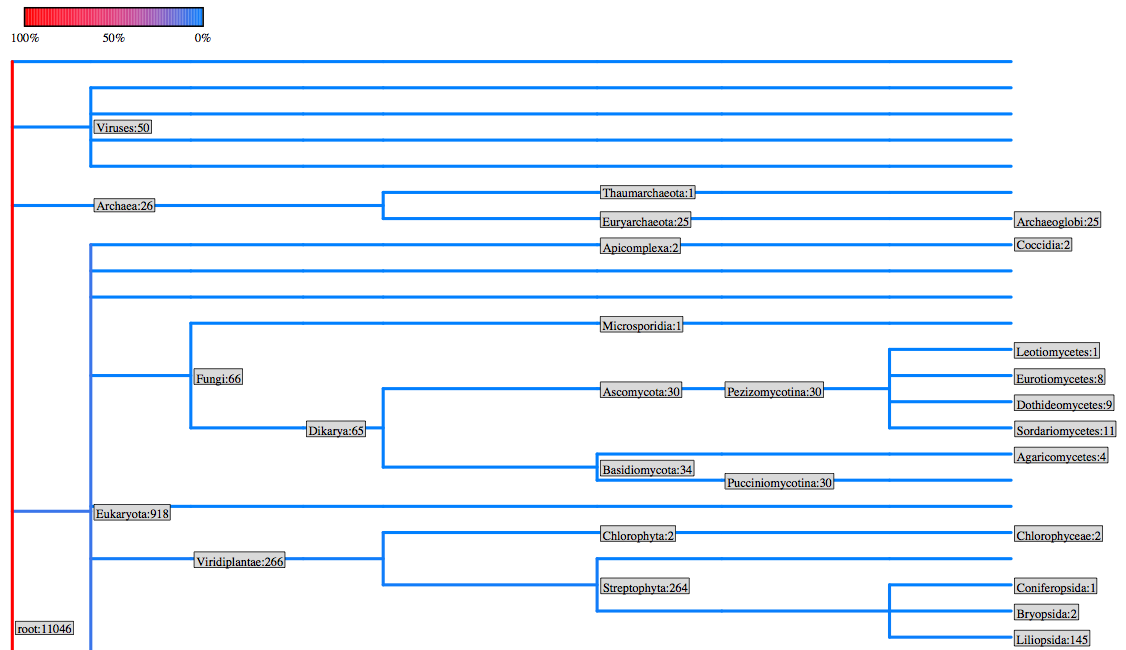
\includegraphics[scale=0.2]{img/resultat.png}
 	\caption{Résultat du workflow}
   \end{center}
  \end{figure}
\end{frame}

\end{document}
